\documentclass[a4paper,11pt,oneside]{report}
\usepackage[table,xcdraw, x11names,dvipsnames,table]{xcolor}

\usepackage{longtable}
\usepackage[utf8]{inputenc}
\usepackage[english]{babel}
\usepackage{courier}
\usepackage{placeins}
\usepackage{amssymb}
\usepackage{amsmath}
\usepackage{graphicx}
\usepackage{tcolorbox}
\usepackage{listings}
\usepackage{graphics}
\usepackage{color}
\usepackage{lipsum}
\usepackage{csquotes}
\usepackage{graphicx}
\usepackage[left=2.00cm, right=2.00cm, top=2.00cm, bottom=2.00cm]{geometry}
\usepackage{array} 
\usepackage{ltablex}
\usepackage{longtable}
\usepackage[strict]{changepage}
\usepackage{tikz}
\usepackage{etoolbox}
\usepackage{multirow}
\usepackage{setspace} 
\usepackage{outlines}
\usepackage{tikz}  %burbujas de texto
\usepackage{textcomp} % si quieres superíndices como "*"
\usepackage[toc,page]{appendix}

% SI NO VAS A USAR GLOSARIO QUITA ESTO
\usepackage{glossaries}    %Glosario
\makeglossaries
\newglossaryentry{raised bed}{
    name=raised bed,
    description={Elevated land surfaces where different crops are cultivated. Their length varies depending on the size of the farms, but they are usually 1.6 meters wide.}
}
\newglossaryentry{slope}{
    name=slope,
    description={Narrow strips of land between the plateaus that allow farmers and tractors to work without damaging the crops.}
	}
\newglossaryentry{transplanted}{
    name=transplanting,
    description={The introduction of plants in their initial stage of development into the soil.
	}
}
\newglossaryentry{Sowing}{
    name=sowing,
    description={Scattering seeds directly onto prepared soil for cultivation.}
}
\newglossaryentry{mesh}{
    name=mesh,
    description={Flexible structures placed over crops to protect the plants from external factors.
	}
}
\newglossaryentry{hoops}{
    name=hoops,
    description={Usually iron arches placed on the plateaus. The mesh is often placed on top, creating a space between the crops and the mesh.
	}
}
\newglossaryentry{harvest}{
    name=harvesting,
    description={Collecting the different products once they have matured.}
}




%\item Plateau: Elevated land surfaces where different crops are cultivated. Their length varies depending on the size of the farms, but they are usually 1.6 meters wide.
		
%\item Slope: Narrow strips of land between the plateaus that allow farmers and tractors to work without damaging the crops.

%\item Planting: The introduction of plants in their initial stage of development into the soil.

%\item Sowing: Scattering seeds directly onto prepared soil for cultivation.

%\item Mesh: Flexible structures placed over crops to protect the plants from external factors.

%\item Hoops or arches: Usually iron arches placed on the plateaus. The mesh is often placed on top, creating a space between the crops and the mesh.

%\item Harvesting: Collecting the different products once they have matured. % definiciones externas

% -----------------------------------------




\usepackage{hyperref}
\hypersetup{
    colorlinks=true,
    linkcolor=grey3,
    filecolor=magenta,      
    urlcolor=azul5,
    pdfpagemode=FullScreen,
    }
\urlstyle{same}



\newcommand{\burbuja}[2]{%
    \tikz[baseline=(bubble.center)]{
        \node[draw, fill=blue!20, text width=#1, align=center, rounded corners] (bubble) {#2};
    }%
}

\DeclareUnicodeCharacter{2212}{-}

% SI NO VAS A USAR BIBLIOGRAFIA QUITA ESTO
\usepackage[backend=biber]{biblatex}
\addbibresource{dummy.bib}
% -----------------------------------------

\usepackage{booktabs}

%Los colores están enumerados de menos a mas tono y saturación
% PALETA DE COLORES: https://www.rapidtables.com/web/color/RGB_Color.html
\definecolor{azul1}{RGB}{204, 229, 255}
\definecolor{azul2}{RGB}{153, 204, 255}
\definecolor{azul3}{RGB}{102, 178, 255}
\definecolor{azul4}{RGB}{51, 153, 255}
\definecolor{azul5}{RGB}{0, 128, 255}
\definecolor{azul6}{RGB}{0, 102, 204}
\definecolor{azul7}{RGB}{0, 76, 153}
\definecolor{azul8}{RGB}{0, 51, 102}
\definecolor{azul_lila1}{RGB}{204, 204, 255}
\definecolor{azul_lila2}{RGB}{153, 153, 255}    
\definecolor{azul_lila3}{RGB}{102, 102, 255}
\definecolor{azul_lila4}{RGB}{51, 51, 255}
\definecolor{azul_lila5}{RGB}{0, 0, 255}
\definecolor{azul_lila6}{RGB}{0, 0, 204}
\definecolor{azul_lila7}{RGB}{0, 0, 153}
\definecolor{azul_lila8}{RGB}{0, 0, 102}

\definecolor{purple_ubuntu}{RGB}{0.172, 0.000, 0.118}
\definecolor{purple_blue}{RGB}{142,170,219}
\definecolor{rojo}{RGB}{224, 59, 35}
\definecolor{grey1}{RGB}{238, 237, 237}
\definecolor{grey2}{RGB}{180, 178, 177}
\definecolor{grey3}{RGB}{67,75, 77}

%Colores terminal
\definecolor{terminal-bg}{rgb}{0.2, 0.2, 0.2}  % Fondo oscuro
\definecolor{terminal-fg}{rgb}{1.0, 1.0, 1.0}  % Texto blanco
\definecolor{terminal-green}{rgb}{0.5, 1.0, 0.5} % Verde para el usuario
\definecolor{terminal-blue}{rgb}{0.4, 0.5, 1.0} % Azul para el directorio

%Caja de la terminal
\newtcolorbox{terminalbox}{colback=terminal-bg, colframe=terminal-bg, 
  boxrule=0pt, left=3pt, right=3pt, top=3pt, bottom=3pt, 
  sharp corners, boxsep=5pt, width=\linewidth}


% Definir comando para formatear automáticamente el prompt
\newcommand{\terminalPrompt}[4]{%
   \textbf{\textcolor{terminal-green}{#1}} % Usuario en verde
   \textbf{\textcolor{terminal-fg}{@}}     % Separador en blanco
    \textbf{\textcolor{terminal-blue}{#2}}  % Host en azul
    \textbf{\textcolor{terminal-fg}{:}}
    \textbf{\textcolor{terminal-blue}{$\thicksim$}}
    \textbf{\textcolor{terminal-blue}{#3}}
    \textbf{\textcolor{terminal-fg}{\$}}   % Separador en blanco
    \textcolor{terminal-fg}{#4}    % Resto del texto en blanco
}


\tcbuselibrary{listings,breakable}
\setlength{\parskip}{3mm}
\tcbset{colback=red!5!white,colframe=red!75!black,size=small,
fonttitle=\bfseries,box align=top}
\lstdefinestyle{customc}{
  breaklines=true,
  language=python,
  basicstyle=\footnotesize\ttfamily,
  keywordstyle=\bfseries\color{purple!40!black},
  commentstyle=\itshape\color{green!40!black},
  identifierstyle=\color{blue},
  stringstyle=\color{orange},
}



\begin{document}
    \begin{titlepage}
    \begin{center}
        {\Huge \textsc{-------}}

        {\Huge \textsc{-------}}  
        
        {\Huge \textsc{-------}}
        
        {\Large{\textbf{Modeling Laboratory - Group Work. Optimization}}}
        
        \vspace{20mm}
        {\large{ 
          Juan Agustín Lorca García

          Paula Marín Turpín
          
          Andrea Martos García

          Rebeca Molina Bernal
          
          Date: 14 March 2025 
          }}

          \vspace{20mm}
        \begin{figure}[ht]
             \centerline{
\includegraphics[width=10cm,height=10cm]{portada/nuevo_logo_umu.png}}
            \label{logo_umu}
        \end{figure}

        \vspace{20mm}
        {\large {University of Murcia}}
        
        {\large {Faculty of Mathematics}}
        \textcolor{rojo}{\rule{\linewidth}{0.55mm}}
    \end{center}
\end{titlepage}
    {\small
\tableofcontents
\thispagestyle{empty}
}
    \chapter*{Introduction}
\addcontentsline{toc}{chapter}{1. Introduction} % Manual index entry
% Hablar de la empresa
% Hablar del objetivo del trabajo
% Comentar la estructura del documento

PRUEBA GLOSARIO: \gls{tempo}$^{(*)}$


En el mundo actual, donde la eficiencia y la toma de decisiones estratégicas marcan la diferencia entre avanzar o quedarse atrás, la gestión de tareas dentro de una empresa adquiere un papel fundamental.
Muchas veces, detrás de un buen producto o servicio, hay una planificación precisa, una coordinación cuidada y un aprovechamiento óptimo de los recursos disponibles.
En este contexto, las matemáticas, y más concretamente la optimización, se convierten en una herramienta poderosa para transformar la complejidad en soluciones claras y aplicables.

Este trabajo surge con la intención de tender un puente entre el conocimiento teórico y su aplicación práctica en el entorno empresarial.
Hemos elegido como caso de estudio la empresa Intercrop, ubicada en Cartagena, especializada en el sector agroalimentario.
Intercrop destaca por su compromiso con la sostenibilidad y la innovación en la producción agrícola, pero como toda empresa, se enfrenta a retos logísticos y organizativos que requieren soluciones inteligentes.
Intercrop no solo opera a nivel nacional, sino que también mantiene una estrecha relación con el mercado internacional. 
Exporta una parte importante de su producción a distintos países europeos, lo que exige altos estándares de calidad, cumplimiento riguroso de plazos y una logística bien estructurada.
Esta dimensión internacional añade complejidad a su gestión operativa, ya que debe coordinar las tareas agrícolas con los calendarios de transporte, las exigencias fitosanitarias y los compromisos comerciales en el extranjero.
Todo ello convierte a esta empresa en un entorno especialmente interesante para aplicar herramientas de optimización que ayuden a mejorar la planificación y la eficiencia en un contexto real y exigente.

A través de este proyecto, abordaremos el problema de planificación de tareas dentro de la empresa. La meta es diseñar un modelo de optimización que permita organizar de forma eficiente las actividades,
 considerando las restricciones del entorno real: tiempos, recursos limitados, dependencias entre tareas y otros factores logísticos.
Este proceso nos permitirá no solo aportar una propuesta de mejora a la empresa, sino también aplicar de forma práctica los conceptos matemáticos aprendidos en el aula, especialmente en lo que respecta a programación lineal y optimización.
\vspace{10mm}
\begin{figure}[ht!]
    \centering
    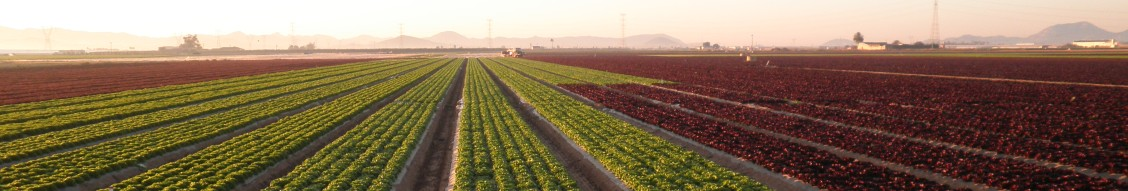
\includegraphics[width=1\textwidth]{img/campitos_lindos.jpeg}
    %\caption{Intercrop, empresa de referencia para el estudio de planificación de tareas agrícolas.}
    \label{fig:campitos_lindos}
\end{figure}

\chapter*{Problem Statement}
\addcontentsline{toc}{chapter}{2. Problem Statement} % Manual index entry
% Explicación en "leguaje natural" del problema
% Simplificaciones
% Descripción de las tareas

La planificación de tareas en el entorno agrícola representa un desafío logístico y operativo considerable,
especialmente en empresas que operan bajo un modelo de producción bajo pedido, como es el caso de Intercrop.
Esta empresa, situada en Cartagena y especializada en productos hortícolas, organiza su producción en función de la demanda estacional.
Durante la campaña de verano, se establecen con antelación tanto la cantidad de kilogramos de producto que se deben suministrar como las fechas específicas de entrega.
Esto implica que toda la planificación de cultivo, desarrollo, cosecha y distribución debe estar ajustada con precisión para cumplir los plazos,
garantizar la calidad del producto fresco (con una vida útil de entre siete y diez días) y minimizar los costes operativos.

El objetivo de este trabajo es abordar, desde un enfoque matemático y práctico, el problema de planificación de tareas agrícolas en el entorno real de esta empresa.
Para ello, nos centraremos en dos cultivos principales: lechuga y espinaca, cada uno con dos variantes específicas.
\begin{itemize}
    \item \textbf{Lechuga}: se cultiva en dos variedades, una de hoja rizada (Apollo, Fig. \ref{fig:apollo}) y otra de hoja lisa (Knox Cos, Fig. \ref{fig:knox}). La lechuga de hoja rizada es más delicada y requiere un cuidado especial. Por su parte, la lechuga de hoja lisa es más resistente y se adapta mejor a condiciones menos precisas.
    \item \textbf{Espinaca}: también se cultiva en dos variedades, una de hoja pequeña (Baby Spinach, Fig. \ref{fig:baby}) y otra de hoja mediana (Teen Spinach, Fig. \ref{fig:teen}). En cuanto a las difere en el tratamiento, no se encuentran ambios sustanciales en el cuidado.
\end{itemize}

\begin{figure}[ht!]
    \centering

    \begin{minipage}[b]{0.45\textwidth}
        \centering
        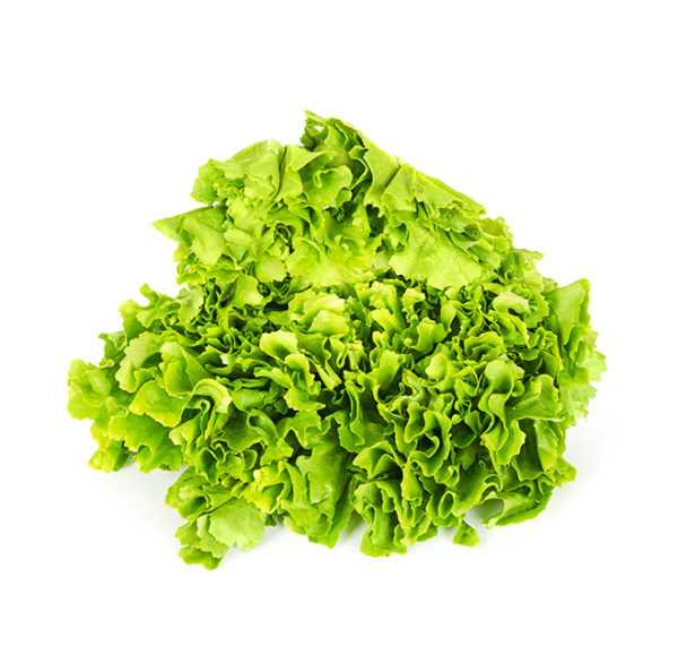
\includegraphics[width=0.7\textwidth]{img/lechuga_apollo.png}
        \caption{Variedad Lechuga Apollo.}
        \label{fig:apollo}
    \end{minipage}
    \hfill
    \begin{minipage}[b]{0.45\textwidth}
        \centering
        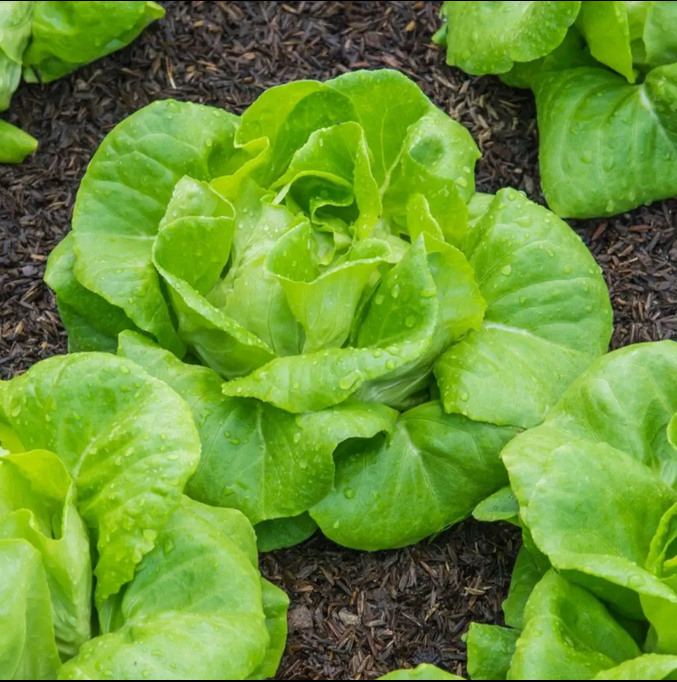
\includegraphics[width=0.6\textwidth]{img/lechuga_knox.png}
        \caption{Variedad Lechuga Knox Cos.}
        \label{fig:knox}
    \end{minipage}

\end{figure}

\begin{figure}[ht!]
    \centering

    \begin{minipage}[b]{0.45\textwidth}
        \centering
        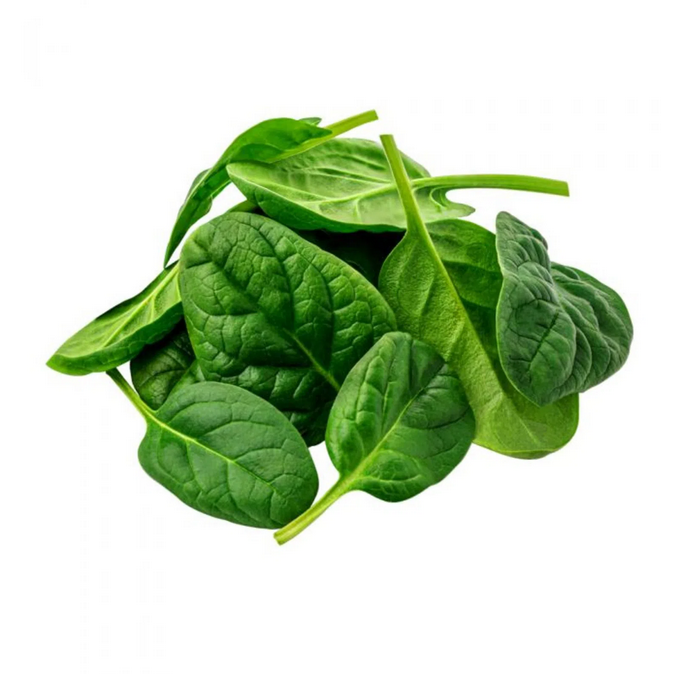
\includegraphics[width=0.7\textwidth]{img/baby_spinach.png}
        \caption{Variedad Baby Spinach.}
        \label{fig:baby}
    \end{minipage}
    \hfill
    \begin{minipage}[b]{0.45\textwidth}
        \centering
        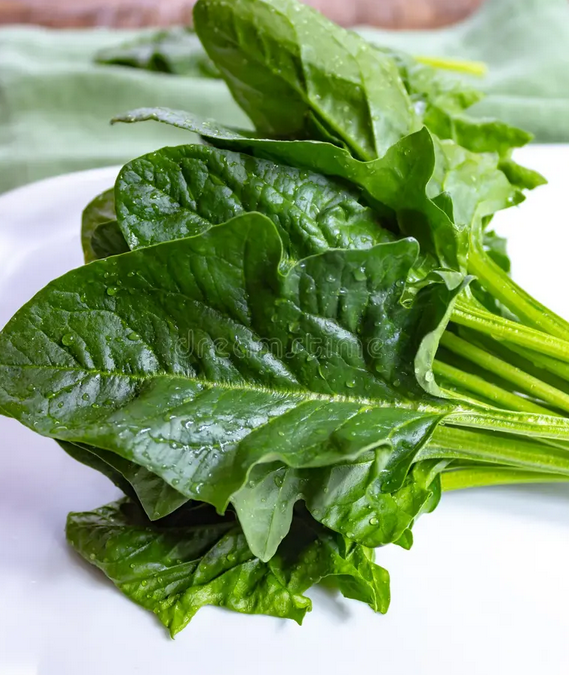
\includegraphics[width=0.6\textwidth]{img/teen_spinach.png}
        \caption{Variedad Teen Spinach.}
        \label{fig:teen}
    \end{minipage}

\end{figure}


Antes de pasar a desglosar las tareas que engloban el poceso de cultivo, es importante destacar una diferencia fundamental entre ambos productos.
La lechuga se trabaja mediante plantación: las semillas se envían a un semillero y posteriormente se trasplantan las plántulas al campo. 
En el caso de la espinaca, se utiliza el método de siembra directa, introduciendo las semillas directamente en la tierra.
Debido al diferente proceder de ambos métodos, cada cultivo tendrá sus tiempos y necesidades específicas, lo que influirá en la planificación de las tareas.

La lista de tareas necesarias para completar un ciclo de cultivo es la siguiente:
\begin{enumerate}
    \item Preparación de la tierra: conjunto de labores inicales donde se rompe y voltea la tierra para airearla, y se abona para dejarla preparada adecuadamente antes del cultivo.
          Seguidamente, mediante maquinaria especializada, se organizan las superficies de cultivo en mesetas.
    \item Colocar papel: se instalan láminas que impiden el crecimiento de malas hierbas, lo que reduce la competencia con el cultivo principal.
    \item Sembrar o plantar: según el tipo de variante, se introducen semillas directamente o se plantan brotes previamente cultivados por una empresa externa.
    \item Riego: instalación de sistemas de riego por aspersión en las laderas de las mesetas, necesarios para el mantenimiento del cultivo.
    \item Colocación de arquillos: se instalan arcos metálicos sobre los cultivos para dar soporte a la protección posterior.
    \item Poner malla: se cubren los arquillos con una malla de poliamida que protege los cultivos y ayuda a mantener la temperatura adecuada para su desarrollo.
    \item Quitar malla: una vez que el cultivo ha madurado, se retira la malla protectora.
    \item Quitar arquillos: tras la retirada de la malla, se procede a desmontar los arquillos metálicos.
    \item Quitar riego: se desmonta el sistema de riego instalado previamente.
    \item Recogida de cosecha: proceso final de recolección, que puede realizarse manualmente (con operarios que colocan los productos en cajas) o de forma automatizada.
\end{enumerate}

Cada una de estas tareas se lleva a cabo con maquinaria distinta, generalmente aperos arrastrados por tractores, lo que implica velocidades de trabajo diferentes según el equipo empleado.
Además, Intercrop organiza su producción mediante grupos de trabajo especializados, que no están contratados desde el inicio de campaña, sino que se van incorporando según se requieren sus funciones.
Esta estructura permite adaptarse a las necesidades del proceso, pero también genera cuellos de botella cuando un grupo debe esperar a que otro finalice su tarea para continuar.

Durante nuestra visita a la empresa, observamos que esta falta de sincronización entre grupos provoca frecuentes horas muertas: periodos en los que los trabajadores están presentes pero sin poder actuar,
ya que el trabajo anterior aún no ha finalizado. Estas horas, aunque no productivas, computan en el total de horas trabajadas y generan un coste económico directo para la empresa.

La presente propuesta tiene como objetivo central la creación de un modelo de planificación que permita minimizar las horas improductivas entre grupos de trabajo,
garantizando al mismo tiempo que se cumplan los plazos de entrega comprometidos. Una coordinación más eficiente de las tareas supondría una mejora significativa en la utilización de los recursos,
reduciendo tiempos de espera y aumentando la productividad general del sistema.

\section*{Simplificaciones del modelo}
\addcontentsline{toc}{section}{2.1. Simplificaciones del modelo} % Manual index entry

Para poder abordar el problema dese un punto de vista matemático y computacional, ha sido necesario realizar algunas simplificaciones, que nos permiten centrarnos en los aspectos esenciales del proceso
sin pérdida de generalidad:
\begin{itemize}
    \item Reducción de escala: el modelo se aplica únicamente a dos fincas, una dedicada a lechuga y otra a espinaca. 
          Esta decisión permite trabajar con dos líneas de producción diferenciadas y representativas, sin necesidad de modelar toda la operación global de la empresa.
    \item Fincas de tamaño medio: se ha asumido que ambas fincas tienen dimensiones similares y medias, lo que permite aplicar el mismo esquema de planificación
          a cada una sin consideraciones de tamaño o forma específicas.
    \item Cultivo homogéneo: se considera que en una misma finca realizaremos las tareas que necesarias para el cuidado de la variedad más delicada. 
          Por tanto, supondremos que en la finca destinada a las lechugas se realizan todas las tareas de la lista mencionada, y en el caso de las espinacas obviaremos el uso de malla y arquillo. 
          Así, en la primera finca se realizarán las 10 tareas mencionadas anteriormente, mientras en la finca correspondiente a las espinacas solo se realizarań las tareas 1, 3, 4, 9 y 10.
    \item Grupos de trabajo independientes: cada cultivo es atendido por  un grupo de trabajo diferente, con su propia maquinaria y recursos.
          Esto permite tratar ambas líneas de producción de manera paralela y simplificada.
    \item Conversión de unidades: las velocidades de la maquinaria, proporcionadas por la empresa originalmente en kilómteros por hora, han sido traducidas a caminos por hora,
          para simplificar la formulación y adaptar las unidades a la estructura del modelo.
    \item Condiciones ideales: el modelo se desarrolla bajo un escenario en el que no hay fallos mecánicos ni interrupciones por causas climáticas.
          Es decir, se asumen que todas las tareas se realizan en el tiempo estimado y que no hay retrasos por factores externos.
    \item Jornada laboral fija: se condidera una jornada laboral de 8 horas diarias, sin cambios estacionales ni festvos.
\end{itemize}
 
Estas simplificaciones no eliminan la complejidad del problema, pero permiten estructurar un modelo realista, funcional y computacionalmente viable que sirva como base para una futura ampliación o implementación práctica.






\chapter*{Formulation}
\addcontentsline{toc}{chapter}{3. Formulation} % Manual index entry
% Variables
% Funcion objetivo
% Restricciones

Para abordar la planificación de tareas agrícolas de manera estructurada y optimizable, hemos construido un modelo matemático que describe formalmente las restricciones, recursos y objetivos del problema planteado.
Esta formulación nos permitirá buscar una asignación eficiente de tareas que minimice los tiempos improductivos, garantizando que las labores se ejecuten de acuerdo a sus requisitos técnicos y temporales.

\section*{Parametros}
\addcontentsline{toc}{section}{3.1. Parámetros} % Manual index entry
Lo primero que necesitamos es definir un conjunto de parámetros que represente correctamente el entorno de trabajo en ambas fincas, cada una dedicada a un producto distinto (lechuga y espinaca),
y por tanto, como se mencionaba anteriormente, con secuencias de tareas diferenciadas.


\subsubsection{Conjunto de tareas}
\begin{itemize}
    \item Conjunto de tareas para la finca 1, destinada a lecuhga:
    
    $T_1$:= \{preptierra1,papel1,plantar1,ponerriego1,ponermalla1,quitarmalla1,quitarriego1,cosecha1\}
    \item Conjunto de tareas para la finca 2, destinada a espinaca:
    
    $T_2$:= \{preptierra2,sembrar2,ponerriego2,quitarriego2,cosechar2\}
\end{itemize}

\subsubsection{Caminos y horizonte temporal}

Como ambas fincas tienen dimensiones similares, se define un mismo conjunto de caminos ($C$) y horas ($H$) para ambas:
    \[\begin{aligned}
        C:={1....50}\\
        H:={1...240}
    \end{aligned}\]

\subsubsection{Disponibilidad temporal de las tareas}

Las tareas no están activas durante todo el horizonte temporal: van entrando escalonadamente. 
Además, como en cada finca habrá distintnas tareas disponibles, definimos una familia de horarios para cada una:

\[\begin{aligned}
    H_1 &:= \{H_{preptierra1},H_{papel1},H_{plantar1},H_{ponerriego1},H_{ponermalla1},H_{quitarmalla1},H_{quitarriego1},H_{cosecha1}\}\\
    H_2 &:= \{H_{preptierra2},H_{sembrar2},H_{ponerriego2},H_{quitarriego2},H_{cosechar2}\}   
\end{aligned}\]    

\subsubsection{Velocidad de trabajo de las máquinas}

Cada tarea se realiza con maquinaria diferente, y por tanto a diferentes velocidades. Estas se expresan en mesetas/hora:
\begin{center}
$M_{i_1}:=$ numero maximo de mesetas por camino en una hora $\forall i_1 \in T_1$

$M_{i_2}:=$ numero maximo de mesetas por camino en una hora $\forall i_2 \in T_2$
\end{center}


\subsubsection{Personal asociado a cada tarea}
Cada tarea cuenta con un grupo de trabajo asignado, que incluye un número de personas necesario para su ejecución.
\begin{center}
    $P_{i_1}$ := número de personas asignadas a la tarea $i_1 \in T_1$

    $P_{i_2}$ := número de personas asignadas a la tarea $i_2 \in T_2$    
\end{center}

\section*{Variables de decisión}
\addcontentsline{toc}{section}{3.2. Variables de decisión} % Manual index entry
Para modelar correctamente la ejecución de las tareas en cada meseta y en cada momento del horizonte temporal, se define la siguiente variable binaria:
\[\begin{aligned}
    x_{i_j,k,l} = \begin{cases} 1 & \text{si la tarea } i \text{ se realiza en el camino } k \text{ y en la hora } l \\ 0 & \text{en otro caso} \end{cases}
\end{aligned}\]

donde:
\begin{itemize}
    \item $i_j$ representa una tarea perteneciente al conjunto $T_j$.
    \item $k \in C$ representa una de las mesetas o caminos disponibles en la finca.
    \item $l \in H_i$ representa una hora dentro del intervalo de disponibilidad de la tarea $i$.
\end{itemize}

Por otro lado, para capturar los tiempos de espera o horas muertas entre tareas
(es decir, cuando un grupo de trabajo está disponible pero no puede comenzar porque otra tarea previa no ha terminado en esa meseta), definimos la siguiente variable:
\[\begin{aligned}
    w_{i_j,l} = \begin{cases} 1 & \text{si la tarea } i \text{ se puede asignar todavía a un camino en la hora } l \\ 0 & \text{en otro caso} \end{cases}
\end{aligned}\] 
donde:
\begin{itemize}
    \item $i_j$ representa una tarea perteneciente al conjunto $T_j$.
    \item $l \in H_{i_j}$ representa una hora dentro del intervalo de disponibilidad de la tarea $i$ de la tierra $j$.
\end{itemize}



\section*{Restricciones}
\addcontentsline{toc}{section}{3.3. Restricciones} % Manual index entry
El modelo de planificación agrícola debe garantizar que la ejecución de las tareas se ajusta a las capacidades operativas,
al calendario disponible y al orden lógico del proceso productivo. Para ello, se han definido las siguientes restricciones:
\begin{itemize}
    \item Cada tarea solo puede cubrir un número máximo de mesetas por hora, en función de la velocidad de la maquinaria utilizada:
          \[
            \sum_{k\in C}x_{i_j,k,l} \leq M_{i_j} \qquad \forall i_1 \in T_1, \qquad l\in H_{i_1} \text{   asociado}
          \]
    \item  Solo podemos realizar las tareas una única vez en los caminos donde se puedan realizar:
          \[
            \sum_{i_1 \in T_1, l\in H_{i_1}}x_{i_1 kl} =1 \qquad \forall k \in C
          \]
    \item Debemos respetar el orden que siguen las tareas:
          \[
            x_{i_j,k,l} \leq \sum_{l' \in h_{prev(1)}, l'<l}x_{prev(1),k,l'} \qquad \forall i_1\in T_1 \rightarrow k\in C, l \in H_{i_1}
          \]
    \item Hay que respetar el crecimiento de cada variedad. Una vez puesto el riego la planta comienza a crecer, y debe pasar un tiempo hasta que crezca.
    El tiempo depende de la variedad. Una vez pasado dicho tiempo, se puede realizar la tarea 'quitar malla'.
          \[
            x_{\text{quitarmalla}1,k,l} \leq \sum_{l'\in H_{\text{ponerriego}1}, l'<l-s_1}x_{\text{ponerriego}1,k,l'} \qquad k\in \{1, ..., 50\}, l\in H_{\text{quitarmalla}1} 
          \]
          Esta misma restricción se da para $s_2$ y en este caso tendríamos que $k \in \{37, ..., 50\}$. 
	
    \item Por último, necesitamos una restricción que active $w_{i_1 l}$, es decir, que nos diga si todavía se puede realizar una tarea en una meseta. 
          \[
          \displaystyle w_{i_1 l}\geq \frac{C_{i_1}-\sum_{l'<l, l'\in H_{i_1}, k\in C}x_{i_1 kl}}{C_{i_1}}
          \]
          
          En el sumatorio se cuentan las mesetas en las que se ha realizado una determinada tarea. Este cociente será $0$ cuando una tarea se haya realizado en todas las mesetas, y será mayor que 0 y menor que 1, cuando todavía quede alguna meseta por hacer. 
\end{itemize}


\section*{Función objetivo}
\addcontentsline{toc}{section}{3.4. Función objetivo} % Manual index entry




\chapter*{Data}
\addcontentsline{toc}{chapter}{4. Data} % Manual index entry
% Explicación de los datos
% Tablas

Durante nuestra visita a la empresa, recopilamos todos los datos necesarios para nuestro análisis. 
Posteriormente, la empresa nos facilitó la información que habíamos solicitado.

Para nuestro estudio, asumimos que las fincas tienen una forma rectangular, con dimensiones promedio
 de 100 x 300 metros. Cada meseta de cultivo mide 1.6 metros de ancho, con surcos laterales de 0.4 metros
  para permitir el paso de la maquinaria. Esto implica que cada camino tendrá unas dimensiones de 2 x 300 metros.
   En consecuencia, en cada finca disponemos de 50 caminos y sus respectivas 50 mesetas para el cultivo.

Dado que todas las tareas están mecanizadas, es fundamental considerar la velocidad de las máquinas utilizadas en el
 proceso. Aunque la empresa nos proporcionó estos datos en kilómetros por hora (km/h), para facilitar nuestra formulación 
 convertimos las unidades a caminos por hora.
 
 \begin{table}[ht!]
    \centering
    \begin{tabular}{|l|c|}
        \hline
        \rowcolor{gray!30} \textbf{\textcolor{grey3}{TASK}} & \textbf{\textcolor{grey3}{SPEED}} \\ 
        \hline
        Soil preparation   & 2  \\ \hline
        Install paper      & 4  \\ \hline
        Plant              & 3  \\ \hline
        Sow                & 4  \\ \hline
        Install irrigation & 3  \\ \hline
        Install hoops      & 3  \\ \hline
        Install mesh       & 3  \\ \hline
        Remove irrigation  & 3  \\ \hline
        Remove mesh        & 4  \\ \hline
        Remove hoops       & 3  \\ \hline
        Harvest seeds      & 3  \\ \hline
        Harvest plants     & 2  \\ 
        \hline
    \end{tabular}
    \caption{Tabla de tareas y velocidades}
    \label{tab:tareas}
\end{table}

Nuestra planificación está diseñada para organizar un mes de trabajo. Considerando una jornada laboral de 8 horas diarias, 
trabajamos con un total de 240 horas al mes.

Por otro lado, los trabajadores se incorporan a la campaña de manera escalonada. Cada uno de ellos está especializado en una 
tarea específica, lo que da lugar a la formación de grupos de trabajo especializados. El número de trabajadores por grupo varía 
en función de la tarea asignada.



\chapter*{Code}
\addcontentsline{toc}{chapter}{5. Code} % Manual index entry\addcontentsline{toc}{chapter}{5. Code} % Manual index entry
% Explicación del código
% Código

\chapter*{Results}
\addcontentsline{toc}{chapter}{6. Results} % Manual index entry
% Explicación de los resultados
% Tablas
% Gráficos

\chapter*{Conclusion}
\addcontentsline{toc}{chapter}{7. Conclusion} % Manual index entry
El presente trabajo ha permitido abordar un problema real de planificación agrícola desde una perspectiva matemática,
aplicando herramientas de optimización para mejorar la organización del trabajo en la empresa Intercrop.
A través del análisis de las distintas tareas necesarias para el cultivo de lechuga y espinaca —dos productos clave en la producción de la empresa—
se ha puesto de manifiesto la complejidad operativa asociada a la coordinación de equipos, maquinaria y tiempos de ejecución.

A lo largo del proyecto se ha desarrollado un modelo simplificado, pero representativo,
que tiene como objetivo principal minimizar las horas improductivas entre los grupos de trabajo.
Este enfoque responde a una problemática observada directamente en campo:
la existencia de tiempos de espera innecesarios cuando una tarea no puede comenzar hasta que otra finaliza.
Estas horas muertas, aunque inevitables en cierta medida, suponen un coste directo para la empresa y reducen la eficiencia global del sistema productivo.

El modelo ha sido construido considerando dos fincas independientes, cada una con su línea de producción,
y una secuencia de tareas que incluye desde la preparación del terreno hasta la recolección.
A pesar de las simplificaciones introducidas —como la homogeneización del tamaño de las fincas,
la ausencia de condiciones climáticas adversas o la separación estricta entre los grupos de trabajo—, el planteamiento conserva una estructura lógica fiel al proceso real,
permitiendo extraer conclusiones prácticas y escalables.

El desarrollo del trabajo ha demostrado cómo los conocimientos matemáticos adquiridos en el aula pueden ser aplicados con éxito a problemas reales,
aportando soluciones concretas y cuantificables a situaciones cotidianas del entorno profesional.
Además, ha abierto una vía interesante para seguir profundizando en el uso de modelos de optimización en contextos agrícolas,
donde las decisiones eficientes pueden traducirse en mejoras significativas de rendimiento y rentabilidad.

En futuras fases, se podrían incorporar elementos adicionales al modelo, como la variabilidad climática,
los imprevistos mecánicos o la disponibilidad parcial de maquinaria y personal.
También sería interesante extender el estudio a varias fincas interconectadas o explorar estrategias de contratación y rotación del personal más flexibles.
Todo ello contribuiría a construir una herramienta aún más robusta para la toma de decisiones en la gestión diaria de empresas como Intercrop.

\newpage
------------------------------

- Topo
- Apero
- Siembra
- Plantación
- Meseta
- Arquillo
- Malla
- Papel
- Farm lanes: caminos entre las mesetas para el paso de la maquinaria.
- Semillero

    
    \printglossaries
    \addcontentsline{toc}{chapter}{A. Glossary} % Manual index entry

    %\printbibliography
\end{document}
